\section{Introduction}
To start development from an existing codebase, developers could fork the repository to take a copy of existing source code, which is common in open source and industry. Developers have the freedom and independence to make modifications on their own fork~\cite{dubinsky2013exploratory, bitzer2006impact, ernst2010code,vetter2007open}. However, many forks of a repository not merge their changes back into the original code base which makes it difficult to keep track of decentralized development activity of all the forks when the number of forks grows. \Luyao{this word comes from INFOX paper originally? should I add cite? It can be easily prove by my tool, or should we prove it ?} Some of the developers on Github we have interviewed previously confirmed the problems they faced in terms of losing overview of forks. For example, one said: \emph{"I do not have much visibility of the forks. They are too many and it is overwhelming to keep track of them."}~\cite{ZSLXWK:ICSE18} It shows that the demand for an overview of forks is really existed on software development platforms like GitHub. The network view and members view was supported on GitHub, but it is difficult to gain an overview of specific activities in many forks. As another developer said: \emph{"The network view is helpful for seeing how active a fork is, but often you have to scroll back a lot to find the fork point and then you have to go to the end again for seeing what changed since then in the parent and in the fork, by reading the tooltips of each commit. And the Members view is just a big list of projects, only helpful for finding the parent of all forks, and for opening all of them in browser tabs to read the descriptions."} \footnote{\url{https://github.com/dear-github/dear-github/issues/175}}
Other related work shows that for fork-based development in industrial contexts it is hard for individual teams to know who is doing what and what code changes are made in other forks~\cite{berger2014three,Duc:2014:FCM:2652524.2652546}. Lack of an overview of forks leads to several problems like redundant development, lost contributions and suboptimal forking point~\cite{dubinsky2013exploratory,stanciulescu2015forked}. \Luyao{add more explaination on these problem?}So it's necessary to give developers a panoramic view for the various forks.

We implement Forks Insight\footnote{\url{http://www.forks-insight.com}} which sets out to understand activities in various forks and provide insights to interested developers including repository's maintainers, ac-hoc users who are interested in the repositories and want to see others' secondary development to prevent redundant development. Based on the related work S. Zhou did before ~\cite{ZSLXWK:ICSE18}, our tool is a light-weight release version and has no limit to programming language.


\section{Forks Insight}

The user interface of Forks Insight is shown in Figure 1. By comparison of the fork with upstream(Here we only consider the unmerged branch, namely, the code which has already merged into master branch will not be included in our tool)\Luyao{add reason here?}, every row in table is on behalf of one fork included its commits, changed files, lines of code changed, representative keywords, last commit time and created time.


Users could login with their own GitHub accounts and load their public repositories(or any other repository they are interested) on GitHub. Our tool will start crawling and analyzing data if the repository is not in our database yet and remind the user when it's finished. \Luyao{delete this line?}

\begin{figure}[H]
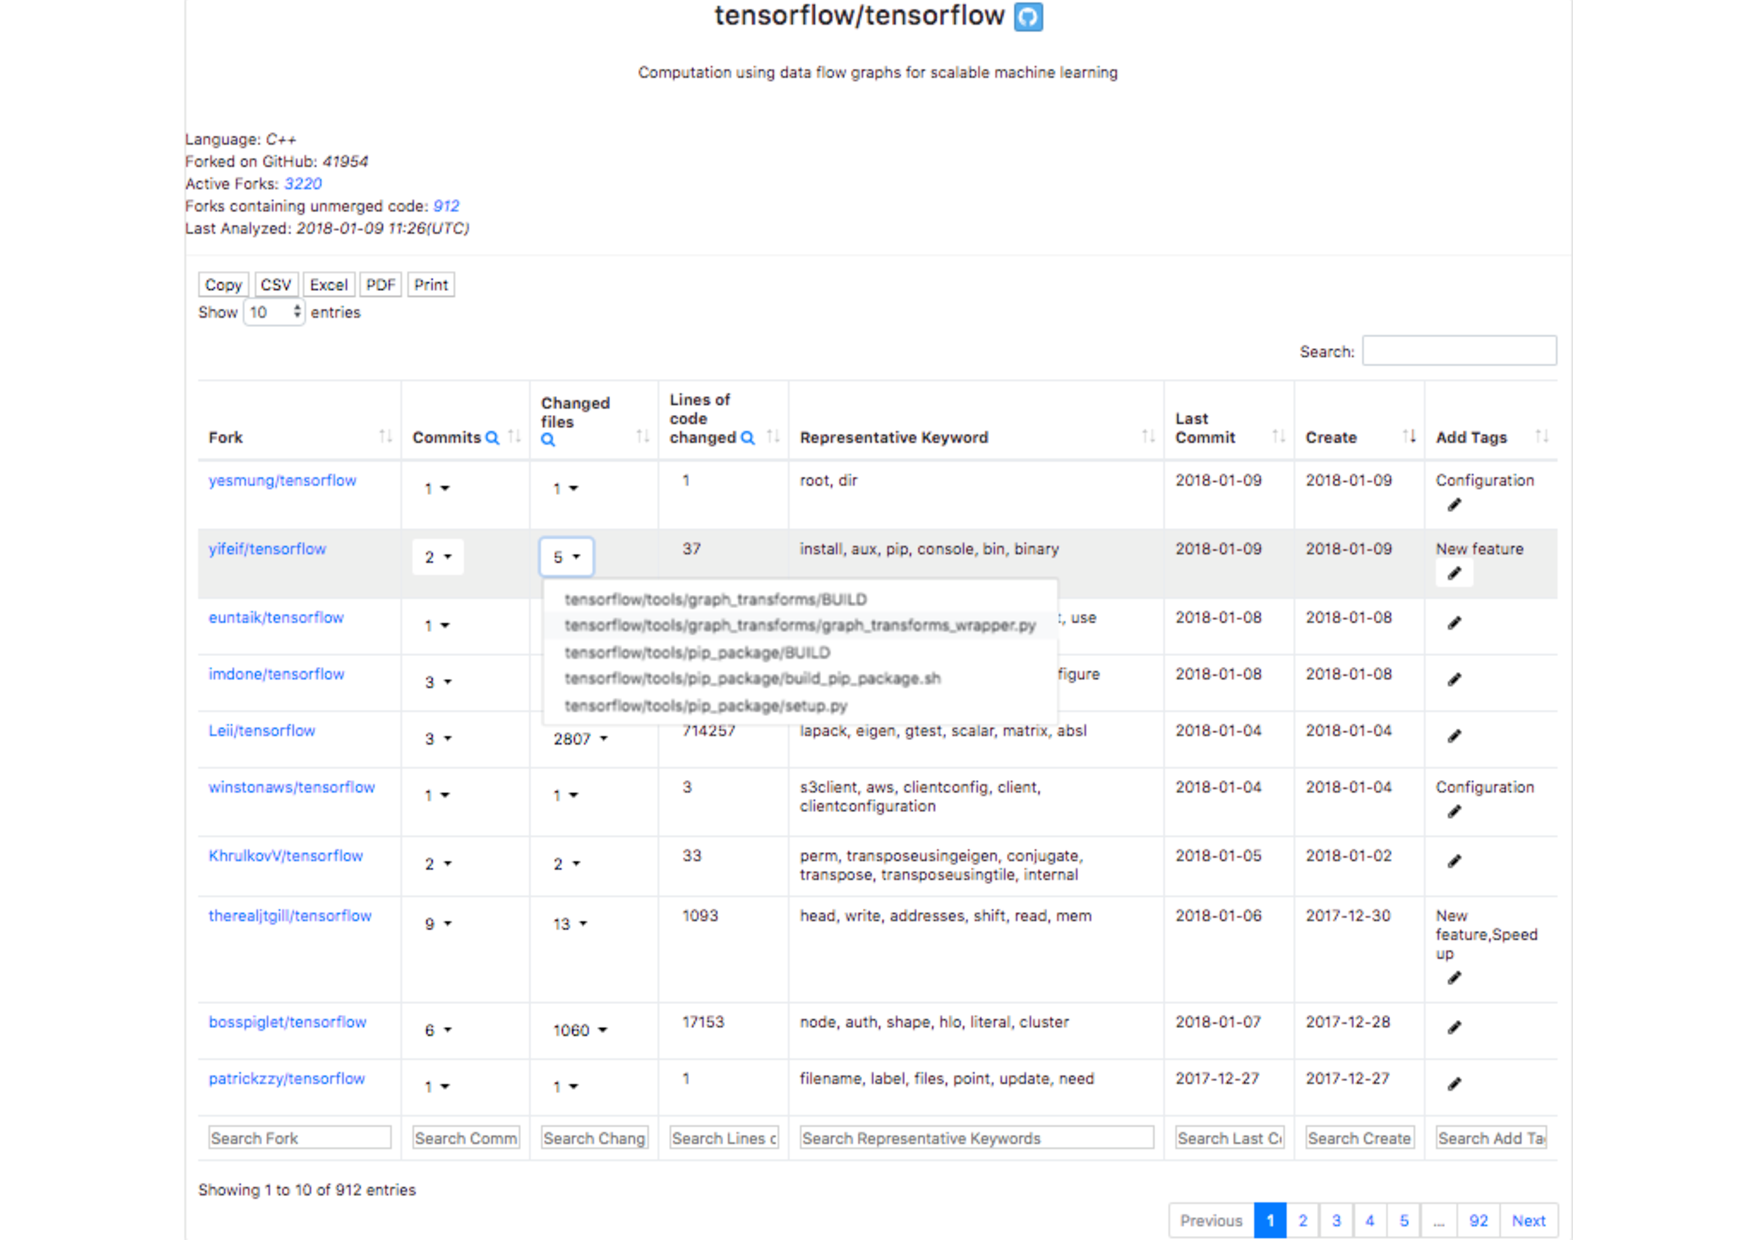
\includegraphics[scale=0.3]{tensorflow_snapshot3.pdf}
\caption{User Interface of Forks Insight.}
\end{figure}

\subsection{Keywords Extract}
As for the column of representative keywords, we use natural language processing on source code, commit messages we fetched. First, we do some preprocessing: remove all the numeric strings; split for underline-separated and Camel-Case cases; lemmatize words to a normal form(for example, the word "dogs" will turn to "dog"). Then, we use TF-IDF ~\cite{salton1988term} to extract keywords from changed code. Though TF-IDF can effectively filter some stop words like "or", "and", there are still some words with high weigh like "public", "private" which is common in language like Java/C++. To improve our result, we manually added the stop words list for different programming language corresponding to their different characteristic.
Fortunately, our method runs fast and has no limit for repository's programming language. Forks Insight can successfully analyze the most popular repositories on Github in hours for the first time.

\subsection{Tagging}
Developers did different developments after forking for different reasons: add new features, fix bugs, change the configuration and so on~\cite{Mikkonen2011,Robles2012,dubinsky2013exploratory,stanciulescu2015forked}.
Since tagging is a simple and intuitive way to summary the characteristic of forks and also convenient to cluster similar forks. So we add a column at the end of each row to allow user to annotate the tags manually on forks. We hope user's contribution on tags can not only help themselves maintain and understand each fork which may reduce the redundant development, but also help the whole open source community, especially for the new users who are interested in this repository but not familiar with repositories. The data of tagging will also be useful for future research work.

\subsection{Retrieval}

\begin{figure}[]
\centering
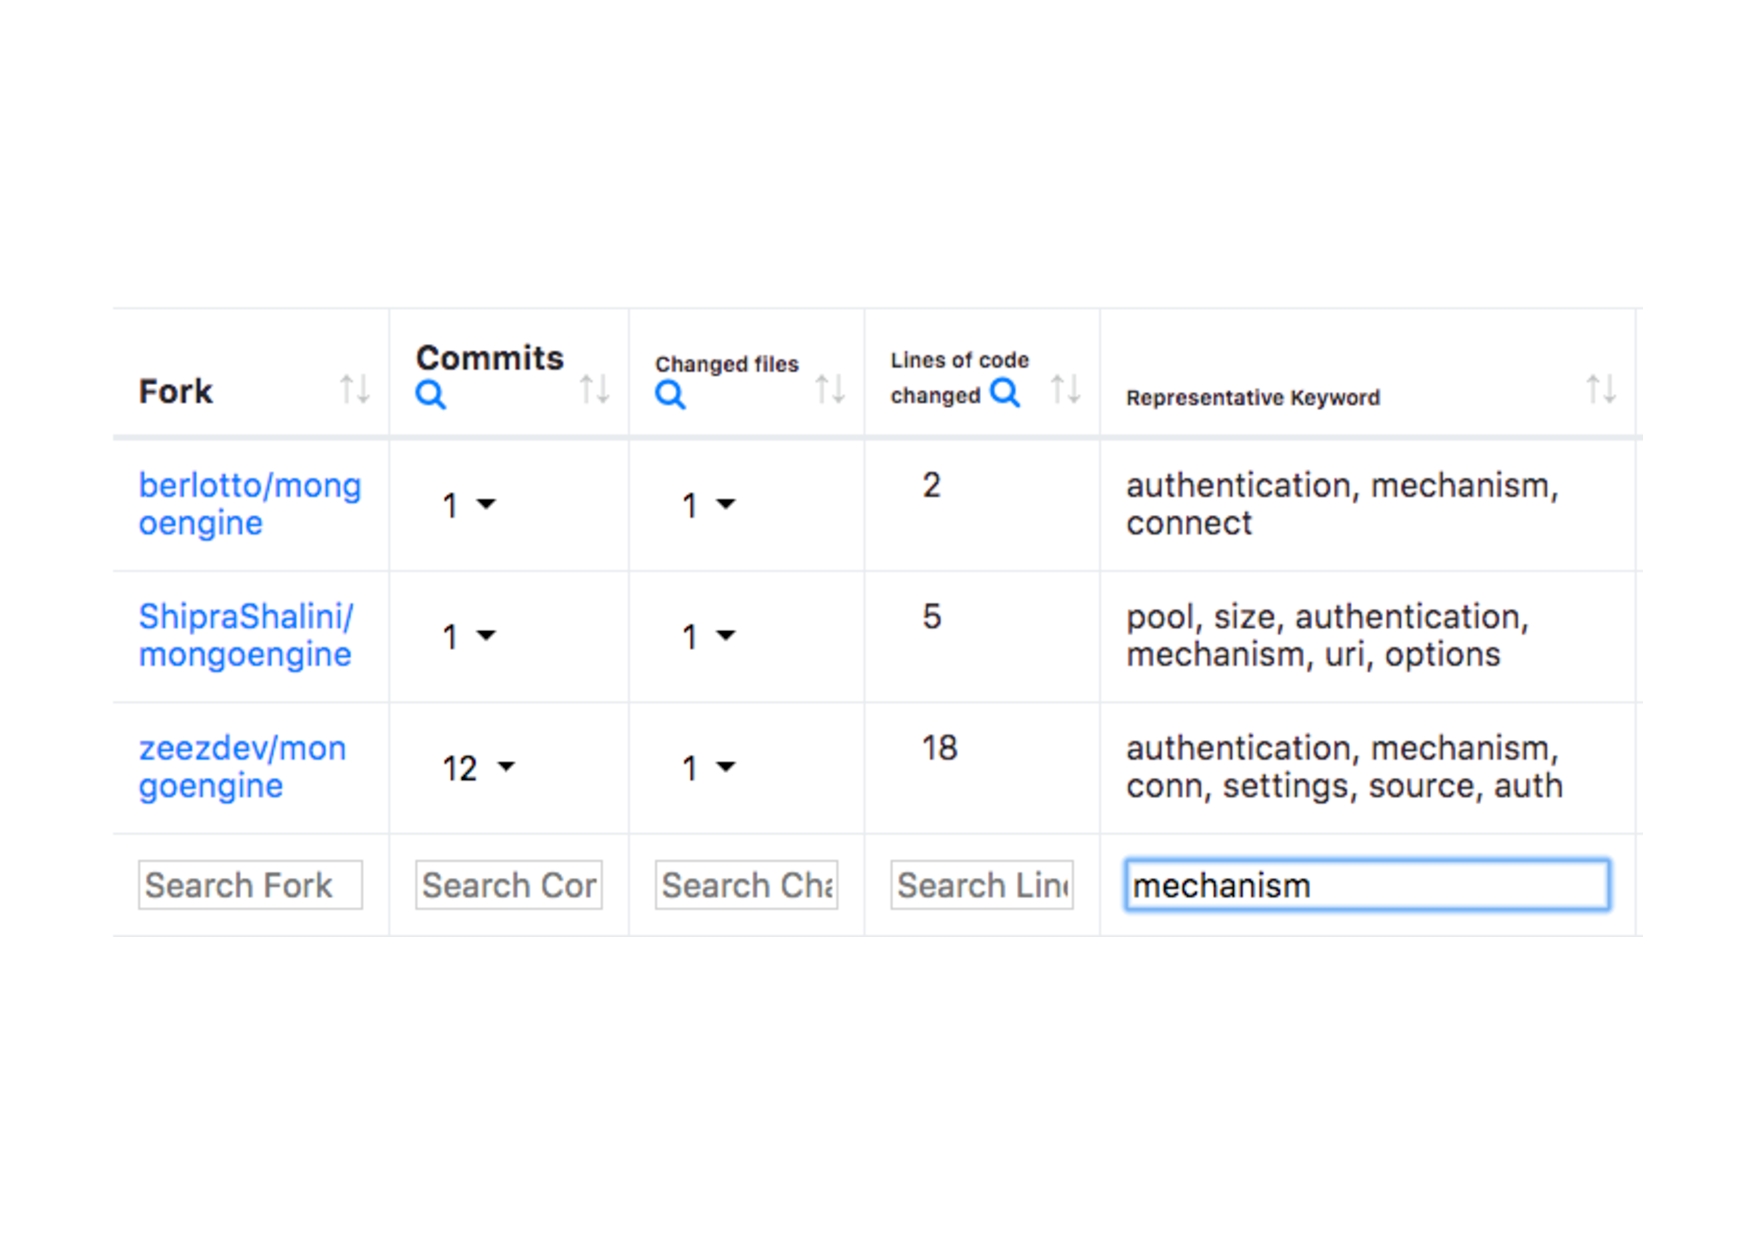
\includegraphics[scale=0.3]{pic5.pdf}
\caption{An example of searching for similar forks.}
\vspace{5pt}
\end{figure}

With the help of the functions like searching, sort, filter in Forks Insight, user can retrieve the forks to dig out useful information. For example, in Figure 2, searching for "mechanism" in forks of MongoEngine\footnote{\url{http://www.forks-insight.com/project/MongoEngine/mongoengine}}, will get three forks which are all related to "mechanism of authentication during connection with database", and contain the same changed file. The example shows that by using keyword search in Forks Insight, user could find out some similar forks which implement or improve the similar thing can effectively \Luyao{or probably?} cut down the possibility of the redundant development.

\section{Conclusions and Future Work}
We implemented a tool to help developers get an overview of the forks to quickly scan and understand them. The current release version focuses on simple analytics for the high level overview which is lightweight, scalable and practical. In order to improve the usability of Forks Insight, we plan to design a user study. And we would like to add more interactive elements and powerful functions on our tool. There are several directions we are considering to move forward: use more visualization to show the meaningful data; identify features in the fork; use natural language to summarize the fork.

\begin{acks}
  TODO
\end{acks}


